We start by identifying points with elements of $\mathbb{R}^2$. Concretely,~\lstinline|abbrev Point := EuclideanSpace ℝ (Fin 2)|.
The next step is to define what it means for a $k$-gon to be \emph{empty} (with respect to a set of points) and \emph{convex}, which we do in terms of \textsf{mathlib} primitives.

\begin{lstlisting}
/-- `EmptyShapeIn S P' means that `S' carves out an empty shape in `P':
the convex hull of `S' contains no point of `P'
other than those already in `S'. -/
def EmptyShapeIn (S P : Set Point) : Prop :=
    ∀ p ∈ P \ S, p ∉ convexHull ℝ S

/-- `ConvexPoints S' means that `S' consists of extremal points of its convex hull,
i.e. the point set encloses a convex polygon. -/
def ConvexPoints (S : Set Point) : Prop :=
    ∀ a ∈ S, a ∉ convexHull ℝ (S \ {a})

def ConvexEmptyIn (S P : Set Point) : Prop :=
    ConvexPoints S ∧ EmptyShapeIn S P

def HasConvexEmptyKGon (k : Nat) (S : Set Point) : Prop :=
    ∃ s : Finset Point, s.card = k ∧ ↑s ⊆ S ∧ ConvexEmptyIn s S
\end{lstlisting}

Assume for now\footnote{The definition is presented in~\Cref{sec:triple-orientations}.} a predicate \lstinline|Point.ListInGenPos| that states that a list of points is in \emph{general position}, i.e., no three points lie on a common line.
With this we can already state the main theorem of our paper.

\begin{lstlisting}
theorem hole_6_theorem (pts : List Point) (gp : Point.ListInGenPos pts)
    (h : pts.length ≥ 30) : HasConvexEmptyKGon 6 pts.toFinset
\end{lstlisting}

At the root  of the encoding of Heule and Scheucher is the idea that the~\lstinline|ConvexEmptyIn| predicate can be determined by analyzing only triangles. In particular, that a set $s$ of $k$ points in a pointset $S$ form an empty convex $k$-gon if and only if all the ${k \choose 3}$ triangles induced by vertices in $s$ are empty with respect to $S$. This is discussed informally in~\cite[Section 3, Eq.~4]{emptyHexagonNumber}.
Concretely, we prove the following theorem:
\begin{lstlisting}
theorem ConvexEmptyIn.iff_triangles {s : Finset Point} {S : Set Point}
    (sS : ↑s ⊆ S) (sz : 3 ≤ s.card) :
    ConvexEmptyIn s S ↔
    ∀ (t : Finset Point), t.card = 3 → t ⊆ s → ConvexEmptyIn t S
\end{lstlisting}
\begin{figure}
    \centering
    \begin{subfigure}{0.45\textwidth}
        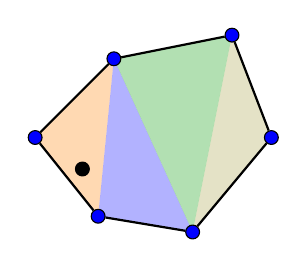
\begin{tikzpicture}
        \coordinate (a) at (0,0);
        \coordinate (b) at (1, 1);
        \coordinate (c) at (2.5, 1.3);
        \coordinate (d) at (3, 0);
        \coordinate (e) at (0.8, -1);
        \coordinate (f) at (2, -1.2);

        \fill[orange, opacity=0.3] (a) -- (b) -- (e) -- (a) -- cycle;
        \fill[blue, opacity=0.3] (b) -- (f) -- (e) -- (b) -- cycle;
        \fill[green!60!black, opacity=0.3] (b) -- (c) -- (f) -- (b) -- cycle;
        \fill[yellow!60!black, opacity=0.3] (c) -- (d) -- (f) -- (c) -- cycle;

        \node[draw, circle, black, fill=blue, inner sep=0pt, minimum size=5pt] (pA) at (0, 0) {};
        \node[draw, circle, black, fill=blue, inner sep=0pt, minimum size=5pt] (pB) at (1, 1) {};
        \node[draw, circle, black, fill=blue, inner sep=0pt, minimum size=5pt] (pC) at (2.5, 1.3) {};
        \node[draw, circle, black, fill=blue, inner sep=0pt, minimum size=5pt] (pD) at (3, 0) {};
        \node[draw, circle, black, fill=blue, inner sep=0pt, minimum size=5pt] (pE) at (0.8, -1) {};
        \node[draw, circle, black, fill=blue, inner sep=0pt, minimum size=5pt] (pF) at (2, -1.2) {};

        \node[draw, circle, black, fill=black, inner sep=0pt, minimum size=5pt] (pG) at (0.6, -0.4) {};


        \draw[thick] (pA) -- (pB) -- (pC) -- (pD) -- (pF) -- (pE) -- (pA);
        % \draw[dashed, thick, red] (pA) -- (pB) -- (pE) -- (pA);
        % \draw[dashed, thick, blue] (pB) -- (pF) -- (pE) -- (pB);
        % \draw[dashed, thick, green!60!black] (pB) -- (pC) -- (pF) -- (pB);


        \end{tikzpicture}
        \caption{}
    \end{subfigure}
    \begin{subfigure}{0.45\textwidth}
        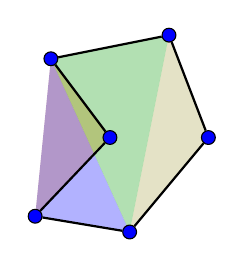
\begin{tikzpicture}
            \coordinate (a) at (1.75,0);
            \coordinate (b) at (1, 1);
            \coordinate (c) at (2.5, 1.3);
            \coordinate (d) at (3, 0);
            \coordinate (e) at (0.8, -1);
            \coordinate (f) at (2, -1.2);

            \fill[orange, opacity=0.3] (a) -- (b) -- (e) -- (a) -- cycle;
            \fill[blue, opacity=0.3] (b) -- (f) -- (e) -- (b) -- cycle;
            \fill[green!60!black, opacity=0.3] (b) -- (c) -- (f) -- (b) -- cycle;
            \fill[yellow!60!black, opacity=0.3] (c) -- (d) -- (f) -- (c) -- cycle;

            \node[draw, circle, black, fill=blue, inner sep=0pt, minimum size=5pt] (pA) at (1.75, 0) {};
            \node[draw, circle, black, fill=blue, inner sep=0pt, minimum size=5pt] (pB) at (1, 1) {};
            \node[draw, circle, black, fill=blue, inner sep=0pt, minimum size=5pt] (pC) at (2.5, 1.3) {};
            \node[draw, circle, black, fill=blue, inner sep=0pt, minimum size=5pt] (pD) at (3, 0) {};
            \node[draw, circle, black, fill=blue, inner sep=0pt, minimum size=5pt] (pE) at (0.8, -1) {};
            \node[draw, circle, black, fill=blue, inner sep=0pt, minimum size=5pt] (pF) at (2, -1.2) {};

            % \node[draw, circle, black, fill=black, inner sep=0pt, minimum size=5pt] (pG) at (0.6, -0.4) {};


            \draw[thick] (pA) -- (pB) -- (pC) -- (pD) -- (pF) -- (pE) -- (pA);
            % \draw[dashed, thick, red] (pA) -- (pB) -- (pE) -- (pA);
            % \draw[dashed, thick, blue] (pB) -- (pF) -- (pE) -- (pB);
            % \draw[dashed, thick, green!60!black] (pB) -- (pC) -- (pF) -- (pB);


        \end{tikzpicture}
        \caption{}
    \end{subfigure}
    \caption{Illustration of the proof for \lstinline|ConvexEmptyIn.iff_triangles|. The left subfigure shows how a point inside the polygon implies the point is inside one of the triangles of triangulation of its convex hull. The right subfigure shows how non-convexity implies one of the vertices of the polygon will be inside one of the triangles of the convex hull partition.}\label{fig:triangulation}
\end{figure}

\begin{proof}[Proof sketch]
    We first prove a simple monotonicity lemma: if $\textsf{ConvexPoints}(s)$, then $\textsf{ConvexPoints}(s')$ for every $s' \subseteq s$, and similarly $\textsf{EmptyShapeIn}(s, S) \Rightarrow \textsf{EmptyShapeIn}(s', S)$ for every set of points $S$.
    By instantiating this monotonicity lemma over all subsets $t \subseteq s$ with $|t| = 3$ we get the forward direction of the theorem.
    For the backward direction it is easier to reason contrapositively: if $s$ does not hold the~$\textsf{ConvexPoints}$ predicate, or is not empty w.r.t.~$S$, then we want to show that there is a triangle $t \subseteq s$ that is also not empty w.r.t.~$S$. To see this, let $H$ be the convex hull of $s$, and then by Carath\'eodory's theorem (cf. \lstinline|theorem convexHull_eq_union| from \textsf{mathlib}), every point in $H$ is a convex combination of at most $3$ points in $s$, and consequently, of exactly $3$ points in $s$.
    If $s$ is non-empty w.r.t.~$S$, then there is a point $p \in S \setminus s$ that belongs to $H$, and by Carath\'eodory, $p$ is a convex combination of $3$ points in $s \setminus \{a\}$, and thus lies inside a triangle $t \subseteq s$ (\Cref{fig:triangulation-a}). If $s$ does not hold $\textsf{ConvexPoints}$, then there is a point $a \in s$ such that $a \in \textsf{convexHull}(s \setminus \{a\})$, and by Carath\'eodory again, $a$ is a convex combination of $3$ points in $s$, and thus lies inside a triangle $t \subseteq s \setminus \{a\}$ (\Cref{fig:triangulation-b}).
%     The
%     The forward direction is easy to see, as triangles are always convex, and if $s$ is empty w.r.t.~$S$, then so are the triangles induced by vertices of $s$.
%     Let $T = \{t_1, \ldots, t_{{k \choose 3}}\}$ be all the triangles induced by vertices of $s$.
%    For the backward direction we will need a \emph{triangulation lemma} stating that the convex hull of $s$ can be partitioned into triangles $P = \{t_i, \ldots, t_j\}$, and $P \subseteq T$.
%     To see that if every $t \in T$ is empty w.r.t. $S$ then $s$ is also empty w.r.t. $S$ we can use the contrapositive statement.
    %  Indeed, assume $s$ is not empty w.r.t. $S$, there is a point $p \in S \setminus s$ that lies inside the convex hull of $s$. Because $P$ is a partition of the convex hull of $s$, point $p$ must be inside some $t \in P \subseteq T$.
    %  To see convexity, we can reason contrapositively again. If $s$ is not convex, then there is a point $p \in s$ that lies inside the convex hull of $s$, and thus lies inside a triangle $t \in P$.
\end{proof}

The next section shows how boolean variables can be used to encode which triangles are empty w.r.t.~a pointset, which as the previous theorem shows, can be used to encode the presence or abscence of $k$-holes.

Another key idea required for the proof is that of ``\emph{triangulations}'': given any convex point set $S$ and a line $\overleftrightarrow{ab}$ between vertices of $S$, the convex hull of $S$ is contained in the convex hull of points on each side of $\overleftrightarrow{ab}$. That is:
\begin{lstlisting}
theorem split_convexHull (cvx : ConvexPoints S) :
  ∀ {a b}, a ∈ S → b ∈ S →
    convexHull ℝ S ⊆
    convexHull ℝ {x ∈ S | σ a b x ≠ ccw} ∪
    convexHull ℝ {x ∈ S | σ a b x ≠ cw}
\end{lstlisting}
By using this lemma repeatedly, we can slice up a convex $k$-gon into smaller pieces in any way we like until we get to triangles, thereby showing that convex polygons can be triangulated. We will use this in particular to show that a hexagon can be covered by only 4 triangles, instead of the ${6\choose 3}$ triangles required by the previous lemma.
\begin{figure}
    \centering
    \begin{subfigure}{0.45\textwidth}
        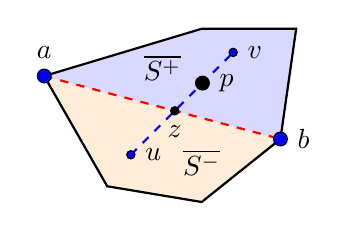
\begin{tikzpicture}
        \coordinate (a) at (0, 0.4);
        \coordinate (b) at (3, -0.4);
        \coordinate (v1) at (3.2, 1);
        \coordinate (v2) at (2, 1);
        \coordinate (u1) at (0.8, -1);
        \coordinate (u2) at (2, -1.2);
        \coordinate (u) at (1.1, -0.6);
        \coordinate (v) at (2.4, 0.7);
        \coordinate (p) at (2.01,0.31);
        \coordinate (z) at (1.65789, -0.0421053);

        \fill[blue, opacity=0.15] (b) -- (v1) -- (v2) -- (a) -- cycle;
        \fill[orange, opacity=0.15] (a) -- (u1) -- (u2) -- (b) -- cycle;

        \draw[thick] (a) -- (u1) -- (u2) -- (b) -- (v1) -- (v2) -- (a);
        \draw[dashed, thick, red] (a) -- (b);
        \draw[dashed, thick, blue] (u) -- (v);

        \node[draw, circle, black, fill=blue, inner sep=0pt, minimum size=5pt, label=above:$a$] (pA) at (a) {};
        \node[draw, circle, black, fill=blue, inner sep=0pt, minimum size=5pt, label=right:$b$] (pB) at (b) {};
        \node[draw, circle, black, fill=blue, inner sep=0pt, minimum size=3pt, label=right:$u$] (pU) at (u) {};
        \node[draw, circle, black, fill=blue, inner sep=0pt, minimum size=3pt, label=right:$v$] (pV) at (v) {};

        \node[draw, circle, black, fill=black, inner sep=0pt, minimum size=5pt, label=right:$p$] (pP) at (p) {};
        \node[draw, circle, black, fill=black, inner sep=0pt, minimum size=3pt, label=below:$z$] (pZ) at (z) {};

        \node[] at (1.5, 0.5) {$\overline{S^+}$};
        \node[] at (2, -0.7) {$\overline{S^-}$};

        \end{tikzpicture}
        \caption{}\label{fig:triangulation2-a}
    \end{subfigure}
    \begin{subfigure}{0.45\textwidth}
        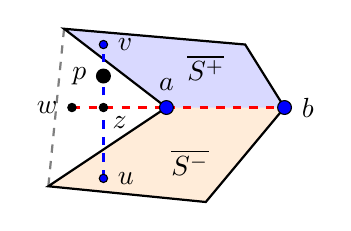
\begin{tikzpicture}
            \coordinate (a) at (1.5, 0);
            \coordinate (b) at (3, 0);
            \coordinate (v1) at (2.5, 0.8);
            \coordinate (v2) at (0.2, 1);
            \coordinate (u1) at (0, -1);
            \coordinate (u2) at (2, -1.2);
            \coordinate (u) at (0.7, -0.9);
            \coordinate (v) at (0.7, 0.8);
            \coordinate (p) at (0.7, 0.4);
            \coordinate (z) at (0.7, 0);
            \coordinate (w) at (0.3, 0);

            \fill[blue, opacity=0.15] (b) -- (v1) -- (v2) -- (a) -- cycle;
            \fill[orange, opacity=0.15] (a) -- (u1) -- (u2) -- (b) -- cycle;

            \draw[thick] (a) -- (u1) -- (u2) -- (b) -- (v1) -- (v2) -- (a);
            \draw[dashed, thick, red] (a) -- (b);
            \draw[dashed, thick, blue] (u) -- (v);
            \draw[dashed, thick, red] (w) -- (a);
            \draw[dashed, thick, opacity=0.5] (v2) -- (u1);

            \node[draw, circle, black, fill=blue, inner sep=0pt, minimum size=5pt, label=above:$a$] (pA) at (a) {};
            \node[draw, circle, black, fill=blue, inner sep=0pt, minimum size=5pt, label=right:$b$] (pB) at (b) {};
            \node[draw, circle, black, fill=blue, inner sep=0pt, minimum size=3pt, label=right:$u$] (pU) at (u) {};
            \node[draw, circle, black, fill=blue, inner sep=0pt, minimum size=3pt, label=right:$v$] (pV) at (v) {};

            \node[draw, circle, black, fill=black, inner sep=0pt, minimum size=5pt, label=left:$p$] (pP) at (p) {};
            \node[draw, circle, black, fill=black, inner sep=0pt, minimum size=3pt, label={[shift={(-0.05,0.05)}]-45:$z$}] (pZ) at (z) {};
            \node[draw, circle, black, fill=black, inner sep=0pt, minimum size=3pt, label=left:$w$] (pW) at (w) {};

            \node[] at (2, 0.5) {$\overline{S^+}$};
            \node[] at (1.8, -0.7) {$\overline{S^-}$};

        \end{tikzpicture}
        \caption{}\label{fig:triangulation2-b}
    \end{subfigure}
    \caption{Illustration of the proof for \lstinline|split_convexHull|. (a) Given point $p$, we obtain points $u$ and $v$ inside the two halves and $z$ as the point of intersection with the line $\overline{ab}$. (b) In this (contradictory) situation, the point $z$ has ended up outside the segment $\overline{ab}$, because $S$ is not actually convex. In this case we construct $w$ such that $z$ is on the $\overline{wa}$ segment, and observe that $w,z,a,b$ are collinear.}\label{fig:triangulation2}
\end{figure}

\begin{proof}
    Let $S^+=\{x\in S\mid \sigma(a,b,x)\ge 0\}$ and $S^-=\{x\in S\mid \sigma(a,b,x)\le 0\}$ be the two sets in the theorem, and let $p\in \overline{S}$, where $\overline{S}$ denotes the convex hull of $S$. Assume WLOG that $\sigma(a,b,p)\ge 0$. (We would like to show that $p\in \overline{S^+}$.) Now $p$ is a convex combination of elements of $S^+$ and elements of $S^-$, so there exist points $u\in \overline{S^-}$ and $v\in \overline{S^+}$ such that $p$ lies on the $\overline{uv}$ line.

    Because $\{x\mid \det(a,b,x)\le 0\}\supseteq S^-$ is convex, it follows that $\det(a,b,u)\le 0$, and likewise $\det(a,b,v)\ge 0$, so they lie on opposite sides of the $\overleftrightarrow{ab}$ line and hence $\overline{uv}$ intersects $\overleftrightarrow{ab}$ at a point $z$. The key point is that $z$ must in fact be on the line segment $\overline{ab}$; assuming that this was the case, we could obtain $z$ as a convex combination of $a$ and $b$, and $p$ as a convex combination of $v$ and $z$, and since $v$ is in $\overline{S^+}$ and $a,b\in S^+\subseteq\overline{S^+}$ we can conclude $p\in \overline{S^+}$.

    To show that $z\in \overline{ab}$, suppose not, so that $a$ lies between $z$ and $b$ (see \Cref{fig:triangulation2-b}). (The case where $z$ is on the $b$ side is similar.) We can decompose $z$ as a convex combination of some $w\in \overline{S\setminus\{a\}}$ and $a$, which means that $w,z,a,b$ are collinear and appear in this order on the line. Therefore $a$ is a convex combination of $w$ and $b$, which means that $a\in \overline{S\setminus\{a\}}$ which violates convexity of $S$.
\end{proof}


% \begin{proof}[Human proof sketch]

% \end{proof}



